\setstretch{1.5}
\section{Θεωρητικό Υπόβαθρο}
\subsection{To μοντέλο Προγραμματισμού \en{OpenMP}}
\subparagraph{}
Το μοντέλο προγραμματισμού του \emph{\en{OpenMP}} βασίζεται στο πολυνηματικό μοντέλο παραλληλισμού.
Η εφαρμογή ξεκινάει με ένα μόνο νήμα, που ονομάζεται κύριο (\emph{\en{master thread}}), που εκτελεί
εντολές σειριακού κώδικα. H ταυτότητα (\emph{\en{id}}) αυτού του νήματος είναι πάντα μηδέν και η
διάρκεια ζωής του είναι μέχρι το πέρας της εκτέλεσης του προγράμματος\cite{pdplab}. 

Όταν το κύριο νήμα  εισέρχεται στην περιοχή παράλληλου κώδικα (\en{parallel region}), τότε
δημιουργούνται περισσότερα νήματα και το τμήμα εκτελείται ταυτόχρονα από τα παραγόμενα νήματα.
Με την ολοκλήρωση της εκτέλεσης του παράλληλου τμήματος, όλα τα νήματα που δημιουργήθηκαν
τερματίζουν και συνεχίζει μόνο το κύριο, μέχρι να βρεθεί κάποιο άλλο τμήμα παράλληλου κώδικα
(\en{fork-join} μοντέλο)\cite{pdplab}. Το κύριο νήμα είναι υπεύθυνο για την δημιουργία των επιπλέον
νημάτων για τη συνολική εκτέλεση. Τα νήματα που είναι ενεργά σε μια παράλληλη περιοχή αναφέρονται ως
\en{"}ομάδα” (\emph{\en{thread team}}). Πάνω από μία ομάδες νημάτων μπορεί να είναι ενεργές
ταυτόχρονα\cite{ompblaise}.

\begin{figure}[h]
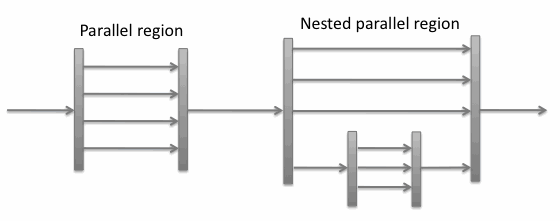
\includegraphics[width=\textwidth]{fork_join}
\captionsetup{justification=centering, singlelinecheck=false}
\caption{Κύριο νήμα και ομάδες νημάτων}
\label{fig:fork_join}
\end{figure}

\subsection{Αλληλεπίδραση νημάτων και περιβάλλοντος δεδομένων}
\subparagraph{}
Οπως προαναφέρθηκε, η εκτέλεση του προγράμματος ξεκινάει από το κύριο νήμα. Το νήμα αυτό
συσχετίζεται με ένα περιβάλλον δεδομένων. Το περιβάλλον δεδομένων για ένα νήμα είναι ο χώρος
διευθύνσεων μνήμης στον οποίο εισάγονται όλες οι μεταβλητές του προγράμματος, περιλαμβανομένων των
\emph{καθολικών} μεταβλητών, των μεταβλητών που είναι αποθηκευμένες στη μνήμη \emph{\en{stack}} και
αυτών που είναι αποθηκευμένες στη \emph{\en{heap}}\cite{book2}. 

Στο μοντέλο μνήμης του \en{OpenMP}, τα δεδομένα χωρίζονται σε δύο βασικές κατηγορίες μνήμης: στα
ιδιωτικά(\emph{\en{private}}) και τα κοινόχρηστα(\emph{\en{shared}}).  Όλα τα νήματα έχουν πρόσβαση
χωρίς περιορισμούς σε μεταβλητές που είναι αποθηκευμένες στην κοινόχρηστη μνήμη\cite{thenextstep7}.

\begin{center}
\begin{figure}[h]
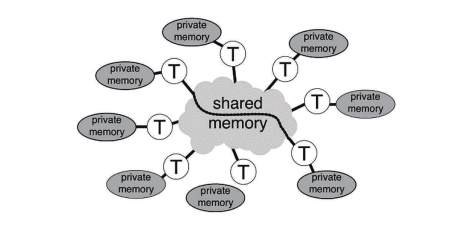
\includegraphics[width=0.9\textwidth]{private_shared}
\captionsetup{justification=centering, singlelinecheck=false}
\caption{Μοντέλο μνήμης \en{OpenMP}}
\label{fig:private_shared}
\end{figure}
\end{center}

\subsubsection{Ιδιωτική μνήμη}
\subparagraph{}
Πρόκειται για τη μνήμη που είναι προσβάσιμη και μπορεί να τροποποιηθεί από ένα μοναδικό νήμα. Κάθε
νήμα δε μπορεί να έχει πρόσβαση στην ιδιωτική μνήμη των υπόλοιπων νημάτων. Η διάρκεια ζωής μιας
μεταβλητής στην ιδιωτική μνήμη είναι περιορισμένη και διαρκεί όσο εκτελείται ο παράλληλος κώδικας.
Από προεπιλογή, κάθε ιδιωτική μεταβλητή δεν είναι αρχικοποιημένη στην αρχή της παράλληλης
περιοχής\cite{thenextstep9}.
\clearpage
\subsubsection{Κοινόχρηστη μνήμη}
\subparagraph{}
Εκτός από την ιδιωτική μνήμη, κάθε νήμα έχει πρόσβαση και σε ένα άλλο είδος μνήμης, την
κοινόχρηστη. Σε αντίθεση με την ιδιωτική, υπάρχει μόνο μία κοινόχρηστη μνήμη κατα τη διάρκεια
εκτέλεσης του προγράμματος, η οποία είναι προσπελάσιμη απο όλα τα νήματα. Ετσι, κάθε νήμα έχει την
δυνατότητα τροποποίησης οποιασδήποτε μεταβλητής βρίσκεται στη κοινόχρηστη μνήμη. Η ταυτόχρονη
προσπέλαση κοινόχρηστης μνήμης από διαφορετικά νήματα, προκαλεί τα παρακάτω προβλήματα:

\paragraph{\en{Race Condition}}
\begin{center}
	\begin{minipage}[t]{0.45\linewidth}
\subparagraph{}
	Το φαινόμενο αυτό εμφανίζεται σε περιπτώσεις που μια ρουτίνα χρησιμοποιεί δεδομένα από τη κοινόχρηστη μνήμη. Αν
αποτελεί τμήμα παράλληλου κώδικα, πολλά νήματα ενδέχεται να προσπαθήσουν να τροποποιήσουν ταυτόχρονα την ίδια διεύθυνση
μνήμης, μέσω αυτής της ρουτίνας. Το πρόβλημα αυτό ονομάζεται \emph{\en{race condition}} και οδηγεί σε εσφαλμένους
υπολογισμούς. 
	\end{minipage}
	\qquad
	\begin{minipage}[t]{0.47\linewidth}
        \selectlanguage{english}
\begin{spacing}{1.1}
\begin{lstlisting}[tabsize=2, basicstyle=\small, language=C++, caption={\el{Παράδειγμα} race condition}, frame=tb]
#include <omp.h>

int main(void) {int sum = 0;

	#pragma omp parallel for
	for (int i = 0;  i < 100; ++i) {
		sum += i;		
	}
}
\end{lstlisting}
\end{spacing}
\selectlanguage{english}
	\end{minipage}
\end{center}
\par
Η απλούστερη λύση, είναι η χρήση της κατάλληλης οδηγίας που επιβάλλει στο πρόγραμμα την προσπέλαση της
μνήμης μόνο από ένα νήμα κάθε χρονική στιγμή. Τέτοιες οδηγίες είναι για παράδειγμα οι \emph{\en{pragma omp
critical/atomic}}. Εναλλακτικά, θα πρέπει αν ειναι εφικτό, να δημιουργείται ιδιωτικού αντίγραφου μεταβλητών για κάθε
νήμα. Έτσι, πολλά νήματα μπορούν ταυτόχρονα να τροποποιούν δεδομένα που βρίσκονται σε διαφορετικές θέσεις μνήμης γιατί
οι μεταβλητές ορίζονται στο ιδιωτικό περιβάλλον δεδομένων του κάθε νήματος.
\clearpage
\paragraph{\en{False Sharing}}
\subparagraph{}
Το \emph{\en{false sharing}} είναι ένα συχνό πρόβλημα στην παράλληλη επεξεργασία κοινόχρηστης μνήμης. Εμφανίζεται όταν
δύο ή περισσότεροι πυρήνες κρατούν αντίγραφο της ίδιας γραμμής προσωρινής μνήμης (\emph{\en{cache}}). 

\begin{figure}[h]
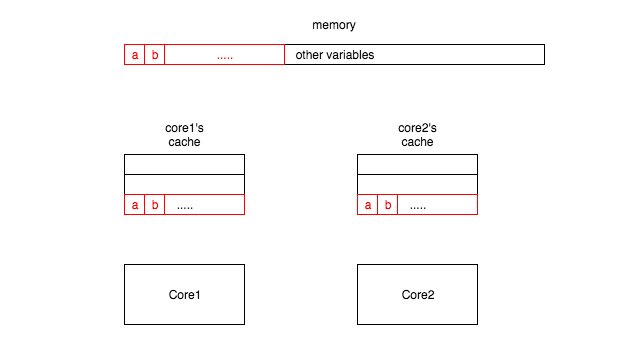
\includegraphics[width=0.6\textwidth]{false_sharing_2}
\centering
\captionsetup{justification=centering, singlelinecheck=false}
	\caption{\en{False sharing (1/3)}}
\label{fig:false_sharing_2}
\end{figure}
\begin{wrapfigure}{l}{0.48\textwidth}
	\centering
	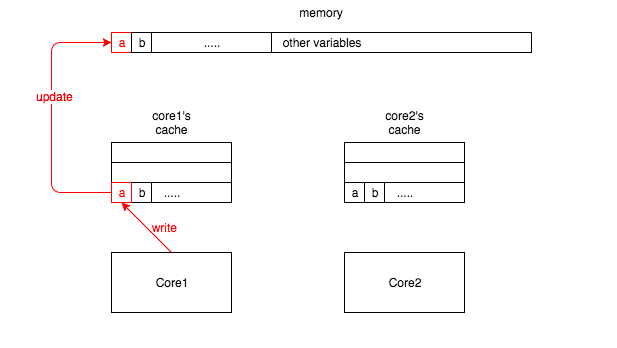
\includegraphics[width=0.5\textwidth]{false_sharing_3}
	\captionsetup{justification=centering, singlelinecheck=false}
	\caption{\en{False sharing (2/3)}}
\label{fig:false_sharing_3}
\end{wrapfigure}
\ \\
Οταν ένα νήμα τροποποιεί μια μεταβλητή, η γραμμή της μνήμης που βρίσκεται η μεταβλητή ακυρώνεται στους υπόλοιπους
πυρήνες. Η γραμμή μνήμης θα πρέπει να ακυρωθεί ακόμη και αν ένας πυρήνας μπορεί να μη τροποποιεί τη συγκεκριμένη θέση
μνήμης, αλλά να θέλει να τροποποιήσει ένα άλλο δεδομένο που βρίσκεται σε αυτή. 

\clearpage

Ο δεύτερος πυρήνας θα πρέπει να φορτώσει εκ νέου τη γραμμή μνήμης, προτού αποκτήσει ξανά πρόσβαση στα δεδομένα της. Η
προσπέλαση δεδομένων της κοινόχρηστης μνήμης συχνά επηρεάζει την απόδοση του προγράμματος\cite{false_sharing}. Λύση στο
πρόβλημα του \en{false sharing}, αποτελεί η εισαγωγή τεχνητού κενού (\en{padding}) ανάμεσα στα δεδομένα της γραμμής, με
σκοπό την τοποθέτησή τους σε ξεχωριστές γραμμές μνήμης.
\ \\

\begin{figure}[h]
    \centering
    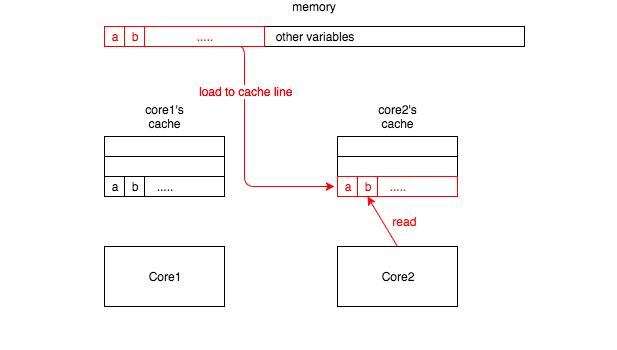
\includegraphics[width=0.6\textwidth]{false_sharing_4}
    \captionsetup{justification=centering, singlelinecheck=false}
	\caption{\en{False sharing (3/3)}}
    \label{fig:false_sharing_4}
\end{figure}
\ \\

\clearpage
\subsection{Αναδρομή σε βασικά χαρακτηριστικά του \emph{\en{OpenMP}}}
\subparagraph{}
Στα κεφάλαια που ακολουθούν αναφέρονται επιγραμματικά βασικές έννοιες και χαρακτηριστικά του \emph{\en{OpenMP}} που
συμπεριλαμβάνονται στην έκδοση 2.5 και χρησιμοποιούνται στα υλοποιημένα παραδείγματα των κεφαλαίων που ακολουθούν. Τα
χαρακτηριστικά αυτά εμπλουτίστηκαν ή προστέθηκαν νέα στις επόμενες εκδόσεις.
\ \\
\subsubsection{Μοντέλο συνοχής μνήμης}
\subparagraph{}
Για την αποφυγή φαινομένων \emph{\en{race condition}} που οδηγούν σε λανθασμένα αποτελέσματα, απαιτείται συχνά ο
συντονισμός πρόσβασης των νημάτων στις μεταβλητές της κοινόχρηστης μνήμης. Ο όρος \emph{"συγχρονισμός"} αναφέρεται σε
τέτοιους μηχανισμούς συντονισμού. Οι οδηγίες συγχρονισμού εγγυώνται την έγγυρη ανάγνωση της σωστής τιμής μιας μεταβλητής
στην κοινόχρηστη μνήμη μετά από οποιαδήποτε ενημέρωσή της. Μηχανισμοί συγχρονισμού ειναι οι εξής\cite{book2_23}:
\selectlanguage{english}
\setlist[1]{itemsep=-2pt}
\begin{itemize}
    \item {\#}pragma omp critical 
    \item {\#}pragma omp atomic
    \item {\#}pragma omp barrier 
    \item {\#}pragma omp ordered
    \item {\#}pragma omp flush
\end{itemize}
\selectlanguage{greek}

\ \\
\subsubsection{Οδηγίες διαμοιρασμού εργασίας}
\subparagraph{}
Η εντολή \textbf{\en{{\#}pragma omp parallel}} κατασκευάζει ένα \textbf{\en{SPMD}} πρόγραμμα (\emph{\en{"Single Program
Multiple Data"}}) όπου κάθε νήμα εκτελεί τον ίδιο κώδικα. Ο όρος \emph{"oδηγία διαμοιρασμού εργασίας"}
(\emph{\en{worksharing construct}}) χρησιμοποιείται για να περιγραφεί η κατανομή της εκτέλεσης της αντίστοιχης περιοχής
κώδικα μεταξύ των νημάτων μιας ομάδας που συναντά την περιοχή αυτή.

Μια οδηγία διαμοιρασμού εργασίας δεν έχει κάποιο υποκείμενο εμπόδιο συγχρονισμού("\emph{\en{barrier}}") κατά την είσοδο
στον τμήμα της παράλληλης περιοχής. Ωστόσο υπάρχει ένας υποκείμενος φραγμός στο τέλος της οδηγίας. Ο φραγμός μπορεί να
αναιρεθεί με τη χρήση της \emph{"φράσης"} \en{(clause)} \textbf{\en{nowait}}. Εάν υπάρχει, το πρόγραμμα θα παραλείψει το
φράγμα στο τέλος της οδηγίας και τα νήματα που ολοκληρώνουν την περιοχή διαμοιρασμένης εργασίας, προχωρούν κατευθείαν
στις επόμενες οδηγίες που ακολουθούν εντός της παράλληλης περιοχής\cite{openmpse16}.
\ \\
\paragraph{Οδηγία διαμοιρασμού εργασίας βρόγχου - \emph{\en{for}}}
\subparagraph{}
Η οδηγία διαμοιρασμού εργασίας βρόγχου καθορίζει ότι οι επαναλήψεις ενός ή περισσότερων βρόχων θα εκτελούνται παράλληλα
από μια ομάδα νημάτων. Οι επαναλήψεις διανέμονται στα ήδη υπάρχοντα νήματα της ομάδας νημάτων της παράλληλης περιοχής. \
\selectlanguage{english}
\begin{spacing}{1.3}
\begin{lstlisting}[language=C++, caption={\el{Σύνταξη οδηγίας διαμοιρασμού εργασίας βρόγχου}} , frame=tlrb]{Name}
#pragma omp for [clause[[,]clause]...] new-line
	for-loops
\end{lstlisting}
\begin{lstlisting}[language=C++, caption={\el{Αποδεκτές φράσεις οδηγίας} for} , frame=tlrb]{Name}
private(list)
firstprivate(list)
lastprivate([lastprivate-modifier:]list)
linear(list[:linear-step])
reduction([reduction-modifier,]reduction-identifier : list)
schedule([modifier[, modifier]:]kind[, chunk_size])
collapse(n)
ordered[(n)]
allocate([allocator :]list)
order(concurrent)
\end{lstlisting}
\end{spacing}
\selectlanguage{greek}

\clearpage
\paragraph{Οδηγία \emph{\en{sections}}}
\subparagraph{}
Η οδηγία \textbf{\en{section}} χρησιμοποιείται για τον μη επαναληπτικό διαμοιρασμό εργασίας σε μια παράλληλη περιοχή.
Καθορίζει ότι τα εσωκλειώμενα τμήματα κώδικα θα διαμοιραστούν μεταξύ των νημάτων της ομάδας. Μια οδηγία
\emph{\en{sections}} μπορεί να περιέχει περισσότερες από μία ανεξάρτητες οδηγίες \emph{\en{section}}. Κάθε
\emph{\en{section}} εκτελείται μια φορά από ένα νήμα της ομάδας και διαφορετικά \emph{\en{sections}} εκτελούνται από
διαφορετικά νήματα. Η σύνταξη μιας οδηγίας \emph{\en{sections}} φαίνεται παρακάτω\cite{pdplab}:
\ \\
\selectlanguage{english}
\begin{spacing}{1.3}
\begin{lstlisting}[language=C++, caption={\el{Σύνταξη οδηγίας} sections} , frame=tlrb]{Name}
#pragma omp sections [clause[ [,] clause] ... ] new-line 
{ 
   [#pragma omp section new-line] 
      structured-block 
   [#pragma omp section new-line 
      structured-block] 
   ... 
   }
\end{lstlisting}
\end{spacing}

\begin{spacing}{1.3}
\begin{lstlisting}[language=C++, caption={\el{Αποδεκτές φράσεις οδηγίας} sections} , frame=tlrb]{Name}
private(list) 
firstprivate(list) 
lastprivate([ lastprivate-modifier:] list) 
reduction([reduction-modifier ,] reduction-identifier : list) 
allocate([allocator :] list) 
nowait
\end{lstlisting}
\end{spacing}
\selectlanguage{greek}

\clearpage
\paragraph{Οδηγία \emph{\en{single}}}
\subparagraph{}
Η οδηγία \textbf{\en{single}} εισάγεται μέσα στην περιοχή παράλληλου κώδικα, με μια ομάδα νημάτων ενεργή και καθορίζει
ότι το εσωκλειόμενο τμήμα σε αυτή την οδηγία εκτελείται από ένα μόνο νήμα, αλλά όχι απαραίτητα από το κύριο. Τα υπόλοιπα
νήματα της ομάδας, παραμένουν αδρανή στο υποκείμενο φράγμα που βρίσκεται στο τέλος της οδηγίας \emph{\en{single}},
εκτός εάν έχει οριστεί η φράση \emph{\en{nowait}}\cite{openmpse16}.

\selectlanguage{english}
\begin{spacing}{1.1}
\begin{lstlisting}[language=C++, caption={\el{Σύνταξη οδηγίας} single} , frame=tlrb]{Name} 
#pragma omp single [clause[ [,] clause] ... ] new-line 
   structured-block
\end{lstlisting}
\end{spacing}

\begin{spacing}{1.1}
\begin{lstlisting}[language=C++, caption={\el{Αποδεκτές φράσεις οδηγίας} sections} , frame=tlrb]{Name}
private(list) 
firstprivate(list) 
copyprivate(list) 
allocate([allocator :] list) 
nowait
\end{lstlisting}
\end{spacing}

\selectlanguage{greek}

\paragraph{Οδηγία \emph{\en{flush}}}
\subparagraph{}
Η οδηγία \textbf{\en{flush}} διασφάλίζει οτι όλα τα νήματα μιας ομάδας στην παράλληλη περιοχή είναι συγχρονισμένα
σχετικά με τις τιμές που υπάρχουν σε συγκεκριμένες μεταβλητές. Η οδηγία \emph{\en{flush}} υπονοείται στις παρακάτω
περιπτώσεις\cite{ibm_flush}:
\setlist[1]{itemsep=-5pt}
\begin{itemize}
\item{\emph{\en{pragma omp barrier}}}
\item{Είσοδος και έξοδος στην οδηγία \emph{\en{omp critical}}}
\item{Έξοδος από την οδηγία \emph{\en{omp parallel}}}
\item{Έξοδος από την οδηγία \emph{\en{omp for}}}
\item{Έξοδος από την οδηγία \emph{\en{omp sections}}}
\item{Έξοδος από την οδηγία \emph{\en{omp single}}}
\end{itemize}

\selectlanguage{english}
\begin{lstlisting}[language=C++, caption={\el{Σύνταξη οδηγίας} flush} , frame=tlrb]{Name} 
#pragma omp flush [memory-order-clause] [(list)] new-line

\end{lstlisting}

\selectlanguage{greek}
\clearpage
\paragraph{Οδηγία \emph{\en{master}}}
\subparagraph{}
Η οδηγία \emph{\en{master}} καθορίζει μια περιοχή κώδικα της παράλληλης περιοχής που εκτελείται μόνο από το κύριο νήμα.
Η χρήση της οδηγίας δεν υπονοεί φράγμα ούτε στην είσοδο αλλά ούτε και στην έξοδο της περιοχής\cite{ibm_master}.


\clearpage
\subsubsection{Φράσεις - \en{Clauses}}
\subparagraph{}
Δεδομένου οτι το \emph{\en{OpenMP}} είναι ένα μοντέλο προγραμματισμού κοινής μνήμης, οι μεταβλητές είναι από προεπιλογή
ορατές από όλα τα νήματα της παράλληλης περιοχής. Οι ιδιωτικές μεταβλητές χρησιμοποιούνται για να
αποφευχθούν φαινόμενα \emph{\en{race conditions}} και υπάρχει ανάγκη μεταβίβασης τους μεταξύ σειριακού κώδικα και
παράλληλης περιοχής με συγκεκριμένες ιδιότητες. Η διαχείριση των δεδομένων επιτυγχάνεται με τη χρήση φράσεων
\textbf{\en{(clauses)}}. Εκτός από τη διαχείριση διαμοιρασμού δεδομένων, υπάρχουν και άλλες κατηγορίες φράσεων που
χρησιμοποιούνται για την διαχείριση της παραλληλοποίησης μέσω \emph{\en{OpenMP}}. Αυτές αναφέρονται στις επόμενες
παραγράφους.
\ \\
\paragraph{Φράσεις διαμοιρασμού δεδομένων - \en{Data sharing attribute clauses}}
\subparagraph{}
Οι φράσεις διαμοιρασμού δεδομένων χρησιμοποιούνται σε οδηγίες για να δώσουν στο χρήστη τη δυνατότητα έλεγχου των
δεδομένων που χρησιμοποιούνται μέσα στην οδηγία.

\subparagraph{\underline{Φράση \en{shared}}}
\subparagraph{}
Η χρήση των μεταβλητών που δημιουργούνται εκτός της παράλληλης περιοχής, επιτρέπεται από όλα τα νήματα. Αν η μεταβλητή
τροποποιηθεί από ένα νήμα, η αλλαγή θα είναι ορατή στα υπόλοιπα νήματα της ομάδας. Οι μεταβλητές με αυτό το
χαρακτηριστικό διατηρούν την τελευταία τιμή τους και μετά την έξοδο από το παράλληλο τμήμα.

\subparagraph{\underline{Φράση \en{private}}}
\subparagraph{}
Τα δεδομένα που δηλώνονται εντός της φράσης είναι ιδιωτικά για κάθε νήμα. Κάθε νήμα θα έχει ένα τοπικό αντίγραφο της
μεταβλητής στην ιδιωτική του μνήμη. Η ιδιωτική μεταβλητή δεν αρχικοποιείται κατα την είσοδο στη παράλληλη περιοχή που
φέρει τη φράση \textbf{\en{private}} και η τελική του τιμή δεν διατηρείται για χρήση εκτός της παράλληλης περιοχής.
\clearpage
\subparagraph{\underline{Φράση \en{default}}}
\subparagraph{}
Δίνει τη δυνατότητα στο χρήστη να δηλώσει ότι η προεπιλογή για τα δεδομένα σε μια παράλληλη περιοχή θα είναι ή
\emph{κοινόχρηστα} ή \emph{\en{none}} για \en{C} / \en{C}++ ή \emph{\en{firstprivate}}. Η επιλογή \emph{\en{none}}
δηλώνει τον υποχρεωτικό ορισμό της κάθε μεταβλητής που χρησιμοποιείται μέσα στην περιοχή παράλληλου κώδικα ως
\en{shared} ή \en{private}, ωστε να καθιστάται σαφές αν θα είναι ιδιωτική ή κοινόχρηστη μέσω των φράσεων διαμοιρασμού
μνήμης που προαναφέρθηκαν.

\subparagraph{\underline{Φράση \en{firstprivate}}}
\subparagraph{}
Η μόναδική διαφορά της φράσης \emph{\en{firstprivate}} από τη \emph{\en{private}} είναι οτι στη πρώτη, η μεταβλητή
αρχικοποιείται χρησιμοποιώντας την τιμή της μεταβλητής που υπάρχει με το ίδιο όνομα εκτός της παράλληλης περιοχής.

\subparagraph{\underline{Φράση \en{lastprivate}}}
\subparagraph{}
Η μοναδική διαφορά της φράσης \emph{\en{lastprivate}} από την \emph{\en{private}} είναι ότι σε αντιθεση με την
τελευταία, η αρχική τιμή ανανεώνεται μετά το πέρας της οδηγίας στην οποία χρησιμοποιήθηκε η συγκεκριμένη φράση. Μια
μεταβλητή μπορεί να είναι δηλωμένη ταυτόχρονα και ως \emph{\en{firstprivate}} αλλά και ως \emph{\en{lastprivate}}.

\subparagraph{\underline{Φράση \en{threadprivate}}}
\subparagraph{}
Η φράση \emph{\en{threadprivate}} ορίζει ότι καθολικά αντικείμενα (ή μεταβλητές) μπορούν να γίνουν προσωρινά ιδιωτικά
για κάποιο νήμα. Με αυτό τον τρόπο, μπορούν δημιουργηθούν καθολικά αντικείμενα, αλλά να μετατρέψουμε την εμβέλειά τους
σε τοπική για κάποιο νήμα. Οι μεταβλητές για τις οποίες ισχύει η φράση \emph{\en{threadprivate}} συνεχίζουν να είναι
ιδιωτικές για κάθε νήμα, ακόμα και σε διαφορετικές παράλληλες περιοχές\cite{pdplab}.
\clearpage
\subparagraph{\underline{Φράση \en{reduction}}}
\subparagraph{}
Εκτελεί μία πράξη αναγωγής για κοινόχρηστες μεταβλητές. Οι μεταβλητές που βρίσκονται σε μία παράλληλη περιοχή και
υπάρχουν στη λίστα της φράσης \emph{\en{reduction}}, μεταφέρονται σε τοπικά αντίγραφα, ένα για κάθε νήμα. Με την
ολοκλήρωση των επαναλήψεων, εφαρμόζεται η πράξη που ορίζεται στο πεδίο \emph{\en{operator}} και το τελικό αποτέλεσμα
αποθηκεύεται στην αρχική θέση τους\cite{pdplab}.
\selectlanguage{english}
\begin{lstlisting}[language=C++, caption={\el{Σύνταξη οδηγίας διαμοιρασμού εργασίας βρόγχου}} , frame=tlrb]{Name}
 reduction(operator | intrinsic : list):\end{lstlisting}
\selectlanguage{greek} 

\ \\
\paragraph{Φράσεις συγχρονισμού - \emph{\en{Data sharing attribute clauses}}}
\subparagraph{}
Σε αυτή την κατηγορία, ανήκουν οι φράσεις που χρησιμοποιούνται για τον συντονισμό των νημάτων μιας ομάδας και την
αποφυγή λανθασμένων υπολογισμών που προκύπτουν από προβλήματα \textbf{\en{race conditions}} σε κοινόχρηστα δεδομένα.

\subparagraph{\underline{Φράση \en{critical}}}
\subparagraph{}
Το τμήμα κώδικα παράλληλης περιοχής που περικλείεται σε αυτή τη φράση, εκτελείται υποχρεωτικά από ένα νήμα κάθε φορά.
Χρησιμοποιείται συχνά για την προστασία κοινόχρηστων δεδομένων από το \emph{\en{race condition}} πρόβλημα.

\subparagraph{\underline{Φράση \en{atomic}}}
\subparagraph{}
H ενημέρωση μνήμης (ανάγνωση-τροποποίηση-εγγραφή) στην οδηγία που ακολουθεί εκτελείται ατομικά. Δεν καθιστά ολόκληρη την
έκφραση \emph{\en{atomic}} αλλα μόνο τις εντολές που αφορούν ενημέρωση μνήμης. Ο μεταγλωττιστής μπορεί να χρησιμοποιεί
ειδικές οδηγίες \emph{\en{hardware}} για καλύτερη επίδοση από ό,τι όταν χρησιμοποιείται το \emph{\en{critical clause}}.
\clearpage
\subparagraph{\underline{Φράση \en{ordered}}}
\subparagraph{}
Σε περιπτώσεις παράλληλου βρόγχου επανάληψης, οι επαναλήψεις εκτελούνται με τη σειρά με την οποία θα εκτελούνταν αν ο
κώδικας ήταν σειριακός.

\subparagraph{\underline{Φράση \en{barrier}}}
\subparagraph{}
Kάθε νήμα περιμένει έως ότου όλα τα άλλα νήματα μιας ομάδας φτάσουν σε αυτό το σημείο. Υπάρχουν οδηγίες, όπως αυτές που
χρησιμοποιούνται για διαμοιρασμό εργασιών βρόγχου, που υπονοούν φράγμα συγχρονισμού \emph{\en{barrier}} στο τέλος της
εκτέλεσης τους.

\subparagraph{\underline{Φράση \en{nowait}}}
\subparagraph{}
Χρησιμοποιείται για να ορίσει ότι τα νήματα που ολοκληρώνουν τη εργασία τους μπορούν να προχωρήσουν στην εκτέλεση εντολών της παράλληλης περιοχής, χωρίς να περιμένουν να τελειώσουν όλα τα νήματα της ομάδας. Ελλείψει αυτής της φράσης, τα νήματα συγχρονίζονται με \emph{\en{barrier}} στο τέλος της οδηγίας.
\subparagraph{\underline{Φράση \en{schedule}}}
\subparagraph{}
Χρησιμοποιείται στην οδηγία διαμοιρασμού εργασίας βρόγχου. Οι επαναλήψεις της οδηγίας ανατίθενται στα νήματα σύμφωνα με τον \emph{τύπο} που ορίζεται μέσα στη φράση.
\selectlanguage{english}
\begin{lstlisting}[language=C++, caption={\el{Σύνταξη οδηγίας διαμοιρασμού εργασίας βρόγχου}} , frame=tlrb]{Name}
schedule(type, chunk): 
\end{lstlisting}
\selectlanguage{greek}
    •  Οι τρεις τύποι \emph{\en{scheduling}} είναι\cite{jakacorner}:\\
\textbf{1. \emph{\en{static}}}:
\subparagraph{}
Οι επαναλήψεις κατανέμονται σε κάθε νήμα πριν την εκτέλεση του βρόγχου και χωρίζονται ισόποσα σε όλα τα νήματα. Η
μεταβλητή \emph{\en{chunk}} αποτελεί έναν ακέραιο που ορίζει τον αριθμό των συνεχόμενων επαναλήψεων που θα εκτελέσει
κάθε νήμα της ομάδας.
\clearpage

Οταν δεν ορίζεται το όρισμα \emph{\en{chunk}}, ο αριθμός των επαναλήψεων που ορίζεται σε κάθε νήμα είναι ίσως με:
$$NumberOfIterations / NumberOfThreads$$
\selectlanguage{english}

\begin{lstlisting}[language=C++, caption={\el{Παραδείγματα φράσης} schedule(static)} , frame=tlrb]{Name}
schedule(static):
T1| ****************                                                
T2|                 ****************                                
T3|                                 ****************                
T4|                                               ****************


schedule(static, 4): 
T1| ****            ****            ****            ****            
T2|     ****            ****            ****            ****        
T3|         ****            ****            ****            ****    
T4|             ****            ****            ****            ****


schedule(static, 8):   
T1| ********                        ********                        
T2|         ********                        ********                
T3|                 ********                        ********        
T4|                         ********                        ********
\end{lstlisting}
\selectlanguage{greek}
\clearpage
\textbf{2. \emph{\en{dynamic}}}: 
\subparagraph{}
Ο τύπος αυτός χρησιμοποιείται όταν από το σύνολο των επαναλήψεων, ένα τμήμα κατανέμεται στα νήματα. Μόλις ένα
συγκεκριμένο νήμα ολοκληρώσει την εκχωρημένη επανάληψή του, συνεχίζει παίρνοντας μία από τις επαναλήψεις που απομένουν.
Το ακέραιο όρισμα \emph{\en{chunk}} καθορίζει τον αριθμό των συνεχόμενων επαναλήψεων που εκχωρούνται σε ένα νήμα κάθε
φορά. Σε περίπτωση που δεν οριστεί αριθμός επαναλήψεων, τότε η προεπιλεγμένη τιμή είναι 1. \ \\
\selectlanguage{english}

\begin{lstlisting}[language=C++, caption={\el{Παραδείγματα φράσης} \emph{schedule(dynamic)} 1/2} , frame=tlrb]{Name}
schedule(dynamic):
T1| *   ** **  * * *  *      *  *    **   *  *  * *       *  *   *  
T2|   *       *     *    * *     * *   *    *        * *   *    *   
T3|  *       *    *     * *   *   *     *  *       *  *  *  *  *   *    
T4|    *  *     *    * *    *  *    *    *    ** *  *   *     *   *                 

schedule(dynamic, 1): 
T1|     *    *     *        *   *    * *  *  *         *  * *  * *  
T2| *  *  *   * *     *  * * *    * *      *   ***  *   *         * 
T3|  *   *  *  *  *    ** *    *      *  *  * *   *  *   *   *  
T4|   *    *     *  **        *  * *    *          *  *    *  * *  *

schedule(dynamic, 4):   
T1|             ****                    ****                    ****
T2| ****            ****    ****            ****        ****        
T3|     ****            ****    ****            ****        ****    
T4|         ****                    ****            ****             
\end{lstlisting}
\clearpage
\begin{lstlisting}[language=C++, caption={\el{Παραδείγματα φράσης} \emph{schedule(dynamic)} 2/2} , frame=tlrb]{Name}
schedule(dynamic, 8):   
T1|                 ********                                ********
T2|                         ********        ********                
T3| ********                        ********        ********        
T4|         ********                                                
\end{lstlisting}
\selectlanguage{greek}

\textbf{3. \en{guided}}: 
\subparagraph{}
Ο τύπος αυτός μοιάζει με τον \emph{\en{dynamic}}. Οι επαναλήψεις χωρίζονται σε ομάδες και κάθε νήμα εκτελεί μια ομάδα
και στη συνέχεια ζητάει την επόμενη για εκτέλεση. Η διαδικασία συνεχίζεται έως ότου δεν υπάρχουν άλλες επαναλήψεις.

Η διαφορά με το δυναμικό τύπο είναι στο μέγεθος των ομάδων που διαχωρίζονται οι επαναλήψεις. Το μέγεθος είναι ανάλογο των μή εκχωρημένων επαναλήψεων διαιρούμενο με τον αριθμό των νημάτων. Επομένως το μέγεθος των ομάδων σταδιακά μειώνεται. Το ελάχιστο δυνατό μέγεθος των ομάδων ορίζεται από το όρισμα \emph{\en{chunk}} του οποίου η προεπιλεγμένη τιμή είναι 1. Παρόλα αυτά, μόνο η τελευταία ομάδα επαναλήψεων μπορεί να είναι μικρότερη από το \emph{\en{chunk}}.

  \selectlanguage{english}
\begin{lstlisting}[language=C++, caption={\el{Παραδείγματα φράσης} \emph{schedule(guided)} 1/2} , frame=tlrb]{Name}
schedule(guided):
T1|                             *********                       
T2|                 ************                     *******  ***   
T3|                                      *******                   *
T4| ****************                            *****       **    * 

schedule(guided, 2): 
T1|                 ************                     ****     **    
T2|                                      *******         ***    **  
T3|                             *********                           
T4| ****************                            *****       **    **
\end{lstlisting}
\begin{lstlisting}[language=C++, caption={\el{Παραδείγματα φράσης} \emph{schedule(guided)} 2/2} , frame=tlrb]{Name}

schedule(guided, 4):   
T1|                                      *******                    
T2|                 ************                     ****    ****   
T3|                             *********                           
T4| ****************                            *****    ****    ***

schedule(guided, 8):   
T1|                 ************                 ********        ***
T2| ****************                                                
T3|                                      ********                   
T4|                             *********                ********
\end{lstlisting}
\selectlanguage{greek}
     
\ \\
\begin{figure}[h]
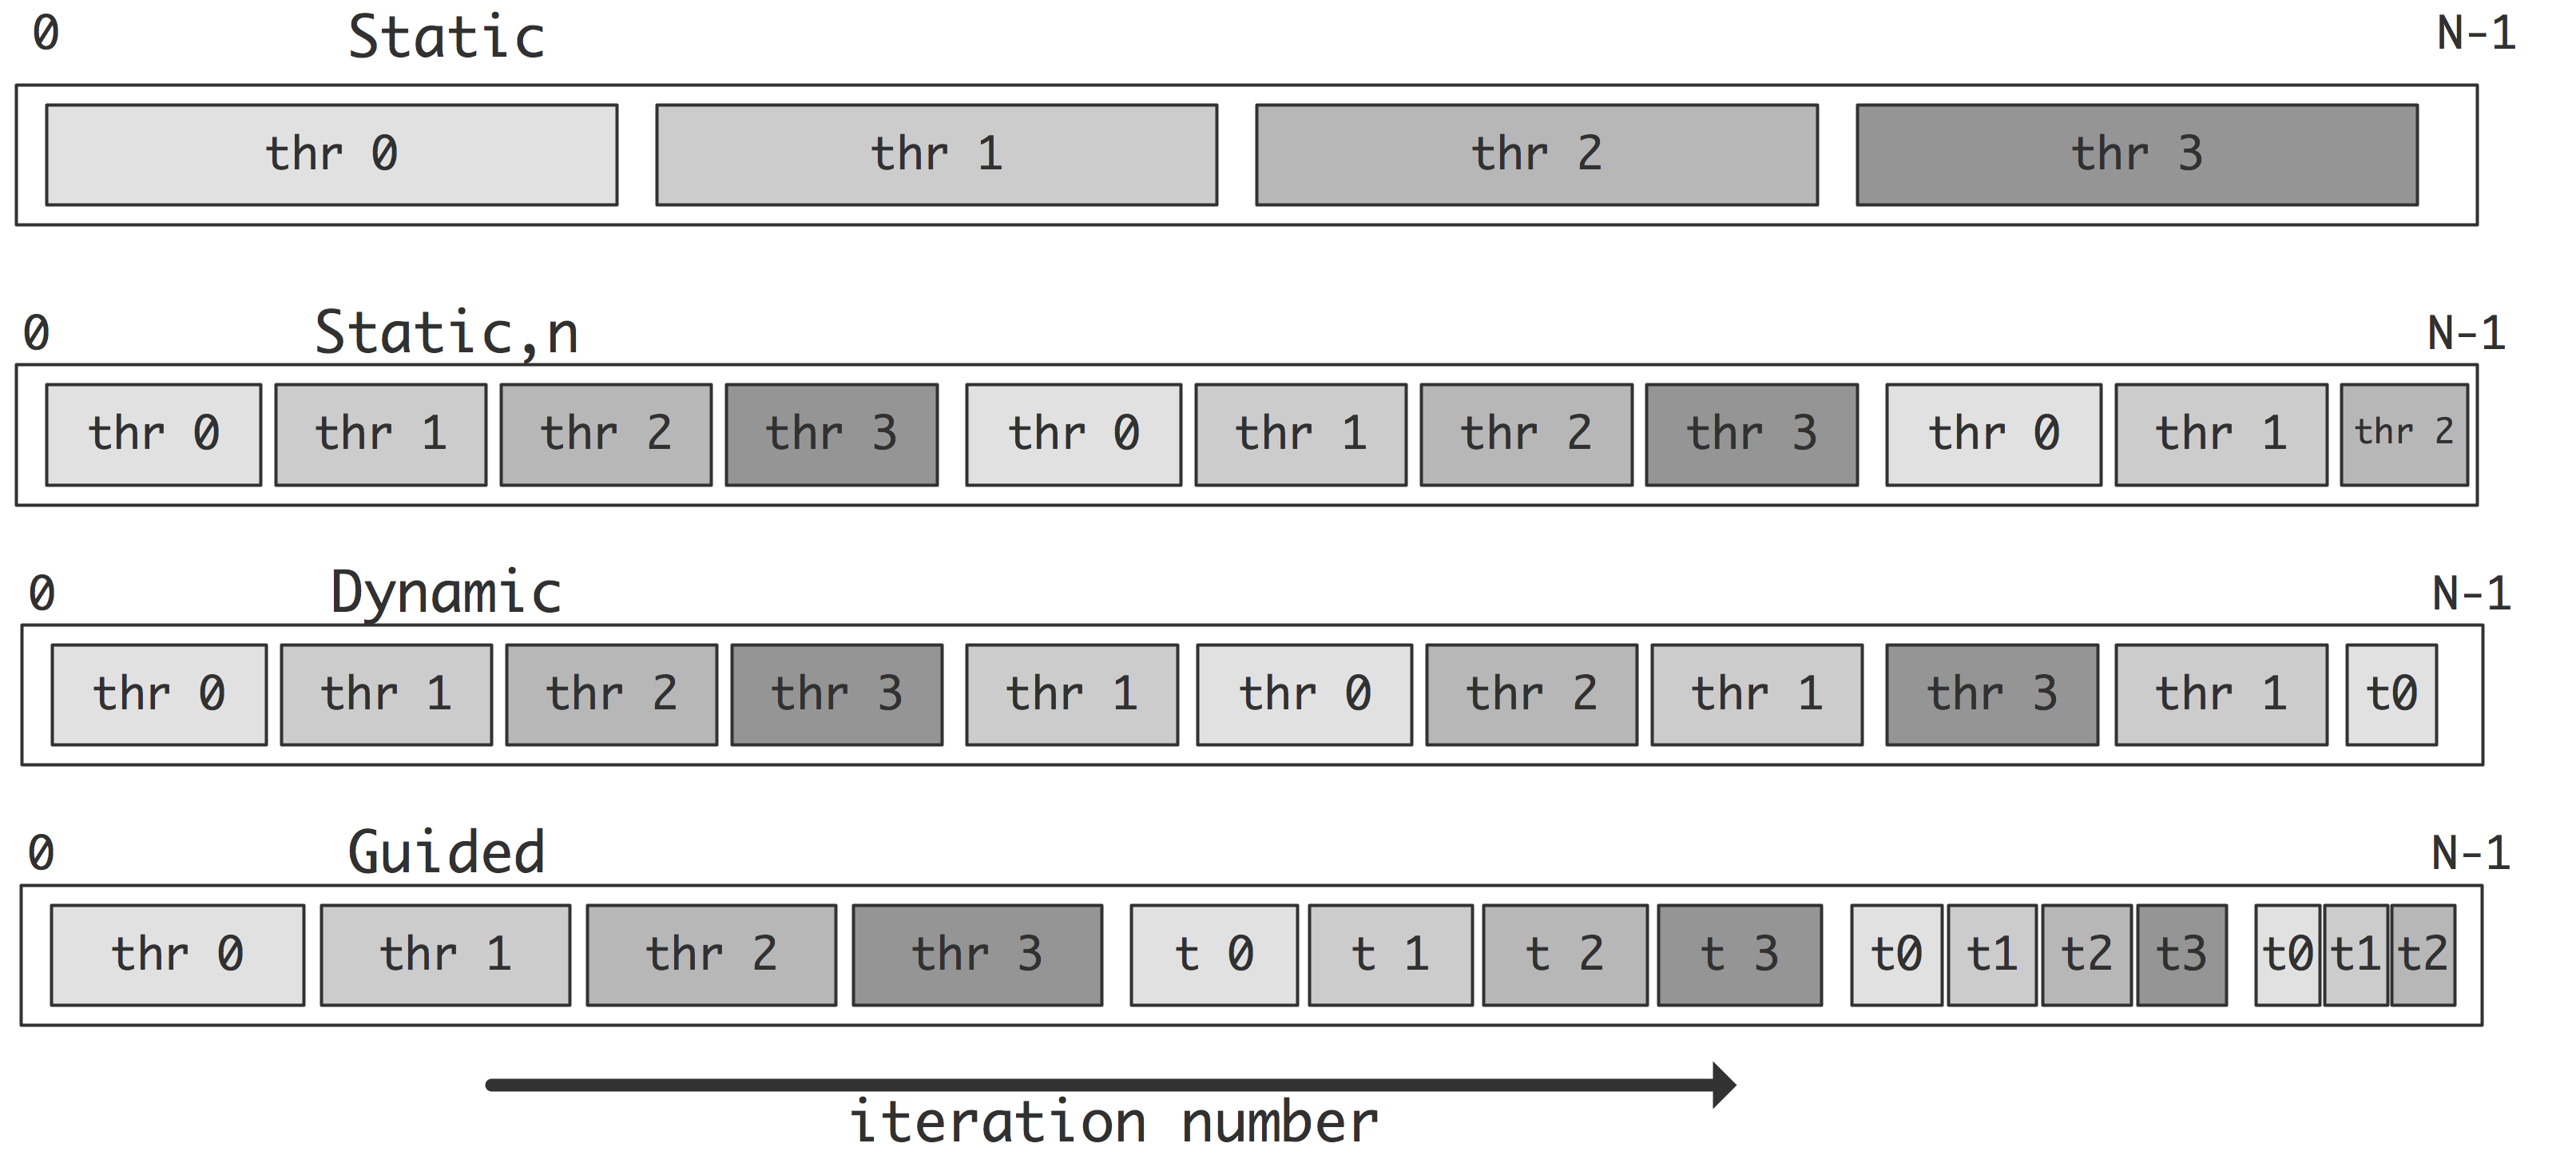
\includegraphics[width=\textwidth]{schedules}
\centering
\captionsetup{justification=centering, singlelinecheck=false}
	\caption{Τύποι φράσης \en{Schedule}}
\label{fig:schedules}
\end{figure}

\clearpage
\subsubsection{Μεταβλητές Περιβάλλοντος}
\subparagraph{}
Για λόγους πληρότητας, η παράγραφος αναφέρεται επιγραμματικά στις μεταβλητές περιβάλλοντος που καθορίζουν τις ρυθμίσεις
των \emph{\en{ICV (Internal Control Variables)}} που επηρεάζουν την εκτέλεση των προγραμμάτων. Τα ονόματα των μεταβλητών
περιβάλλοντος πρέπει να είναι κεφαλαία. Η τροποποίηση των μεταβλητών κατά τη διάρκεια εκτέλεσης του προγράμματος δεν
είναι εφικτή και αγνοείται απο το μεταγλωττιστή. Παρόλα αυτά, μερικές μπορούν να τροποποιηθούν κατα την εκτέλεση
μέσω της χρήσης των αντίστοιχων οδηγίων της διεπαφής\cite{environmental_var}.
\ \\
\begin{table}[htbp]
\captionsetup{justification=raggedright,
singlelinecheck=false
}
\caption{Πίνακας μεταβλητών περιβάλλοντος.}
\def\arraystretch{1.5}
\begin{tabular}{| p{0.5\textwidth} | p{0.5\textwidth}|}
\hline
\emph{\en{OMP\_SCHEDULE}} & \emph{\en{OMP\_NUM\_THREADS}} \\
\hline
 \emph{\en{OMP\_DYNAMIC}} & \emph{\en{OMP\_PROC\_BIND}}\\
\hline
 \emph{\en{OMP\_WAIT\_POLICY}} & \emph{\en{OMP\_NESTED}} \\
\hline
\emph{\en{OMP\_THREAD\_LIMIT}} & \emph{\en{OMP\_MAX\_ACTIVE\_LEVELS}} \\
\hline
\emph{\en{OMP\_CANCELLATION}} & \emph{\en{OMP\_DISPLAY\_ENV}} \\
\hline
\emph{\en{OMP\_DISPLAY\_AFFINITY}} & \emph{\en{OMP\_AFFINITY\_FORMAT}} \\
\hline
\emph{\en{OMP\_DEFAULT\_DEVICE}} & \emph{\en{OMP\_MAX\_TASK\_PRIORITY}} \\
\hline
\emph{\en{OMP\_TARGET\_OFFLOAD}} & \emph{\en{OMP\_TOOL}} \\
\hline
\emph{\en{OMP\_TOOL\_LIBRARIES}} & \emph{\en{OMP\_DEBUG}} \\
\hline
\emph{\en{OMP\_ALLOCATORS}} &  \\
\hline
\end{tabular}
\end{table}

\clearpage
\subsubsection{\emph{\en{Runtime Functions}}}
\subparagraph{}

Σκοπός της παρούσας παραγράφου είναι η συνοπτική αναφορά των ενσωματωμένων ρουτίνων της βιβλιοθήκης
\emph{\en{OpenMP}}. Η κεφαλίδα \textbf{\en{<omp.h>}}, περιλαμβάνει ένα σύνολο ρουτίνων που
χωρίζονται σε τρεις μεγάλες κατηγορίες: 

\begin{itemize}
    \item Τις ρουτίνες ελέγχου περιβάλλοντος εκτέλεσης που χρησιμοποιούνται για τον συντονισμό των νημάτων και της
    εκτέλεσης του παράλληλου τμήματος
    \item Τις ρουτίνες κλειδώματος των νημάτων που χρησιμοποιύνται για τον συγχρονισμό της πρόσβασης στα δεδομένα
    \item Τις ρουτίνες καταμέτρησης χρόνου
\end{itemize}


\begin{table}[htbp]
\captionsetup{justification=raggedright,
singlelinecheck=false
}
\caption{Πίνακας ενσωματωμένων ρουτίνων}
\def\arraystretch{1.5}
\begin{tabular}{| p{0.5\textwidth} | p{0.5\textwidth}|}
\hline
\textbf{Ρουτίνες περιβάλλοντος εκτέλεσης} \cellcolor[HTML]{D0D0D0} & \textbf{Ρουτίνες κλειδώματος} \cellcolor[HTML]{D0D0D0} \\
\hline
 \emph{\en{omp\_set\_num\_threads}} & \emph{\en{omp\_init\_lock}} \\
\hline
\emph{\en{omp\_get\_num\_threads}}  & \emph{\en{omp\_destroy\_lock}} \\
\hline
\emph{\en{omp\_get\_max\_threads}}  &  \emph{\en{omp\_set\_lock}}\\
\hline
\emph{\en{omp\_get\_thread\_num}} &  \emph{\en{omp\_unset\_lock}}\\
\hline
 \emph{\en{omp\_get\_num\_procs}} & \emph{\en{omp\_test\_lock}} \\
\hline
\emph{\en{omp\_in\_parallel}}     & \emph{\en{omp\_init\_nest\_lock}}\\
\hline
 \emph{\en{omp\_set\_dynamic}}    & \emph{\en{omp\_destroy\_nest\_lock}} \\
\hline
 \emph{\en{omp\_get\_dynamic}}    & \emph{\en{omp\_set\_nest\_lock}} \\
\hline
 \emph{\en{omp\_set\_nested}}     &  \emph{\en{omp\_unset\_nest\_lock}}\\
\hline

\hline
      \multicolumn{2}{|c|}{\textbf{Ρουτίνες καταμέτρησης χρόνου}  \cellcolor[HTML]{D0D0D0}}\\
 \hline
\emph{\en{omp\_get\_wtime }}    & \emph{\en{omp\_get\_wtick }} \\
\hline
\end{tabular}
\end{table}



